\chapter{Sequence alignment}

\label{kap:sequence_alignment} % id kapitoly pre prikaz ref

In bioinformatics, a sequence alignment is a way of arranging the sequences of DNA, RNA, or protein
to identify regions of similarity that may be a consequence of functional, structural, or
evolutionary relationships between the sequences. \cite{Gollery2005BioinformaticsSA}

As mentioned in the introduction, sequences are often extremely hard and can't be aligned by human
nor by primitive sequence alignment algorithms. Human knowledge is applied in constructing
algorithms to produce high-quality sequence alignments, and occasionally in adjusting the final
results to reflect patterns that are difficult to represent algorithmically (especially in the case
of nucleotide sequences). Computational approaches to sequence alignment generally fall into two
categories: 

\begin{theorem}[Global alignment]
  Global alignment of two sequences $S_{1}$ and $S_{2}$ requires that the alignment $A$ spans the
  entire length of both the sequences $S_{1}$ and $S_{2}$.
\end{theorem}

\begin{theorem}[Local alignment]
  Local alignment of sequences $S_{1}$ and $S_{2}$ allows the optimal alignment $A$ to span only a
  specific region of the sequences. Local alignments are often used to align a shorter sequence to 
  a larger one.
\end{theorem}

\begin{figure}[H]
  \centerline{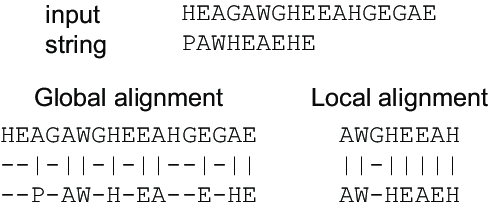
\includegraphics[width=0.8\textwidth]{images/local_global_alignment.png}}
  \caption[Global vs local alignment]{Global vs local alignment}
  \label{obr:local_global_alignment}
\end{figure}

In the following chapter we present the current state of the art algorithms for finding a sequence
alignment (optimal or suboptimal). The algorithms have different properties which vary in the
running time complexity, memory, approximation factor of optimal alignment. Many of the
algorithms don't have scientific guarantees of the optimal solutions and some of the algorithms rely
on the structure of the sequences.

\section{DTW - dynamic time warping}
\label{section:dtw}

Dynamic time warping (DTW) finds similarity between two sequences. It is one of the similarity
methods used in pattern recognition and time series data mining and other fields. The image below
shows an example of non-warping and warping between time series. DTW is efficient similarity method
for time series sequences, but it has quadratic time and memory complexity.

\begin{figure}[H]
  \centerline{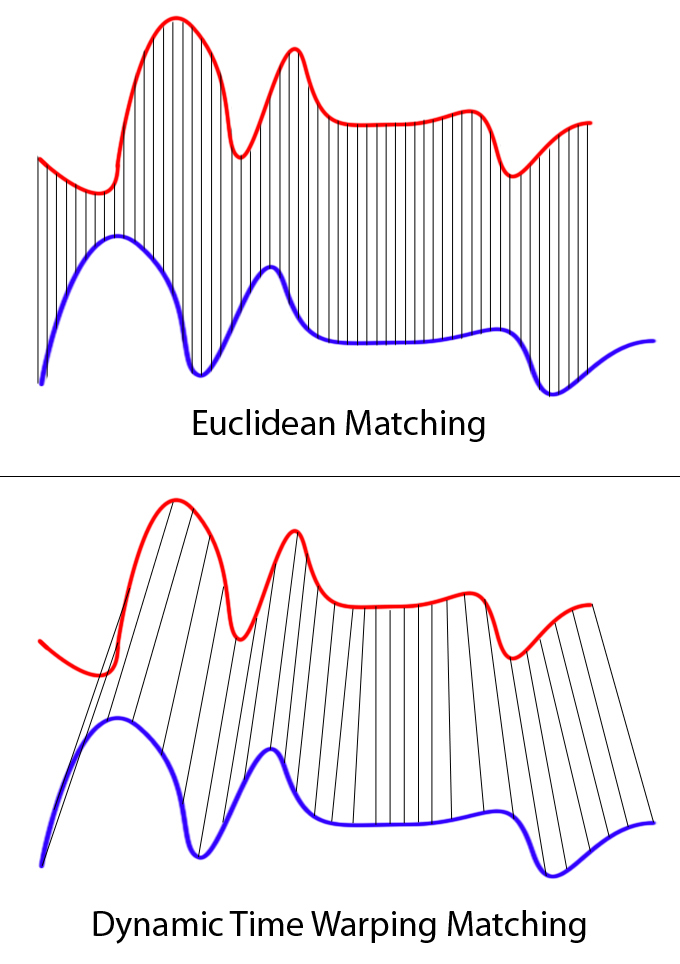
\includegraphics[width=0.4\textwidth]{images/dtw}}
  \caption[DTW]{Warping and non-warping of series}
  \label{obr:dtw}
\end{figure}

The algorithm is pretty straightforward. Suppose we want to calculate the alignment $A$ of two
sequences $S = S_1S_2...S_n$ and $T = T_1T_2...T_m$. Note the lengths of the sequences are $n$ and
$m$, respectively. We will build a matrix $M$ of size $n \times m$, where we will be storing the
score of the alignment (we will later show how to reconstruct the alignment itself). The element
$M[n][m]$ will be the optimal score of the alignment and we will calculate it recursively using the
following algorithm:

\newcommand\numberthis{\addtocounter{equation}{1}\tag{\theequation}}
\begin{align*}
  M[i][j] = \begin{cases}
    i = 0 & j \\
    j = 0 & i \\
    \text{otherwise } & C(S_{i}, T_{j}) + min(M[i-1][j], M[i][j-1], M[i-1][j-1]) \numberthis \label{simple_dtw}
  \end{cases}
\end{align*}

where $C(x, y)$ is a cost function which is defined by:

\begin{align*}
  C(x,y) = \begin{cases}
      x = y & 0 \\
      \text{otherwise } & 1
  \end{cases}
\end{align*}

The algorithm checks all possible operations that can happen \textit{(insertion, deletion, match or
mismatch)}. There is also a variant of the classic DTW algorithm, for which the cost function $C$
returns different values for each type of the operations.

If we want to reconstruct the alignment from the DTW algorithm, we need to create a path matrix $P$
with the same dimensions as $M$. Initially we set $P[i][j] = (i,j)$ for all valid $i, j$. We need to
modify the algorithm \ref{simple_dtw} to store the best option in the path matrix $P$. This defines
the value of $P[i][j]$:

\begin{align*}
  P[i][j] = \begin{cases}
      i = 0 \text{ or } isMin(M[i][j-1]) & (i, j-1) \\
      j = 0 \text{ or } isMin(M[i-1][j]) & (i-1, j) \\
      \text{otherwise} & (i-1, j-1)
  \end{cases}
\end{align*}

where the $isMin(x)$ is a function which returns $true$ if the argument is the best choice (leads to
optimal solution).

The alignment is uniquely represented by the operations which led to the optimal alignment
$M[n][m]$. The operations are linked to each other by the matrix $P$ and can be obtained recursively
starting at value $(n, m)$, following up with $(i,j) = P[n][m]$ until $P[i][j] \ne (i, j)$. The
alignment can be then obtained just by reading the operations in reversed order.

Note that the running time and memory complexity is $n \times m$, because the whole matrix $M$ needs
to be built. This algorithm is usable only for shorter sequences and ignores the biological
properties of the sequences. Sequences in this algorithm could be arbitrary strings and we would
still get the correct and optimal alignment. However, comparing arbitrary strings is not the same as
comparing biological sequences and we might be interested in different scoring methods.

\section{Needleman-Wunsch algorithm}

The Needleman-Wunsch algorithm \cite{NEEDLEMAN1970443}, published in 1970, provides a method of
finding the optimal global alignment of two sequences by maximizing the number of amino acid matches
and minimizing the number of gaps necessary to align the two sequences. When aligning sequences
there are often gaps (i.e. "indels" - insertions and deletions). Biologically, a large gap is more
likely to occur as one large deletion as opposed to multiple single deletions. Hence two small
indels should have a worse score than one large one.

The idea of the algorithm is the same as \ref{section:dtw}. The only difference is the
implementation of cost function, which needs to add additional penalty if there is a gap starting.
You can find more about the gap penalty implementation and further improvements in
\cite{Boes2014ImprovingTN}.

\subsection{BLOSUM}

Needleman-Wunsch algorithm is often used to align protein sequences. There are $20$ standard amino
acids, which are the building blocks of proteins. There are different probabilities that two amino
acids can be aligned together and various penalties if they differ. This led to an idea of
constructing a $20 \times 20$ matrix specifying score for each pair of the acids. 

BLOSUM (\textbf{BLO}cks \textbf{SU}bstitution \textbf{M}atrix) is based on local alignments. BLOSUM
matrices were first introduced in by Steven Henikoff and Jorja Henikoff. They scanned the BLOCKS
database for very conserved regions of protein families (that do not have gaps in the sequence
alignment) and then counted the relative frequencies of amino acids and their substitution
probabilities. Such matrix can be used as a score function to compute optimal alignment in a
biological sense.

\section{DTW performance improvements}

The problem of DTW is that it needs to fill the whole matrix, which is quadratic. We are often
satisfied with near optimal solution as a tradeoff for performance. The methods used make DTW
faster fall into three categories \cite{toward_accurate__dtw}:

\begin{enumerate}
  \item \textbf{Constraints} – Limit the number of cells that are
  evaluated in the cost matrix.
  \item  \textbf{Data Abstraction} – Perform DTW on a reduced
  representation of the data.
  \item  \textbf{Indexing} – Use lower bounding functions to reduce the number of times DTW must be
  run during time series classification or clustering (we will not explain this topic further).
\end{enumerate}

\subsection{Constraints}

Constraints are widely used to speed up DTW. Two of the most commonly used constraints are the
Sakoe-Chuba Band and the Itakura Parallelogram.

\begin{figure}[H]
  \centerline{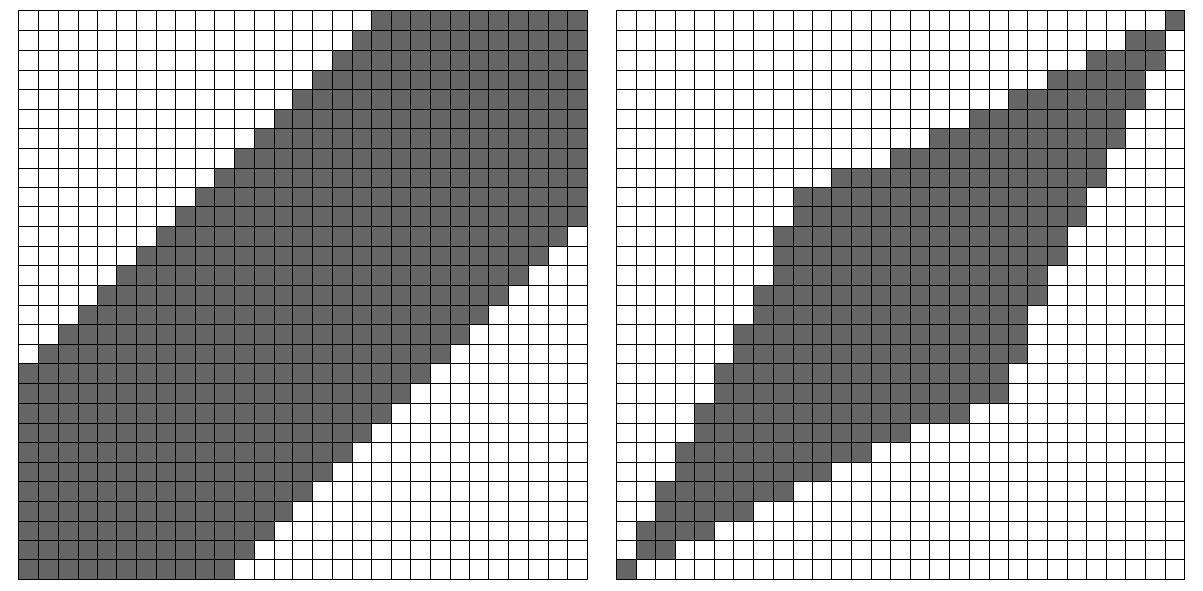
\includegraphics[width=0.7\textwidth]{images/constraints.png}}
  \caption[Two constraints: Sakoe-Chuba Band (left) and an Itakura Parallelogram (right)]{Two
    constraints: Sakoe-Chuba Band (left) and an Itakura Parallelogram (right)}
  \label{obr:constraints}
\end{figure}

The gray cells are the the ones filled by the DTW algorithm. However, the globally optimal warp path
will not be found if it is not entirely inside the window. Using constraints speeds up DTW by a
constant factor, but the DTW algorithm is still $O(N^2)$ if the size of the input window is a
function of the length of the input time series.

Constraints work well in domains where the optimal warp path is expected to be close to a linear
warp and passes through the cost matrix diagonally in a relatively straight line. Constraints work
poorly if time series are of events that start and stop at radically different times because the
warp path can stray very far from a linear warp and nearly the entire cost matrix must be evaluated
to find the optimal warp path. \cite{toward_accurate__dtw}

\subsection{Data Abstraction}

Data abstraction speeds up the DTW algorithm by running DTW on a reduced representation of the data.
Rather than running the DTW algorithm on the full resolution cost matrix, the time series are
reduced in size to make the number of cells in the cost matrix more manageable. A warp path is found
for the lower-resolution time series and is mapped back to the full resolution cost matrix. This
improvement also speeds up the algorithm by a large constant factor, but the running time coplexity
is still $O(N^2)$.

\section{FastDTW}

FastDTW algorithm uses ideas from both the constraints and data abstraction. By combining both of
the DTW improvements it overcomes many limitations of using either method individually, and yields
an algorithm that is linear in both time and space. 

FastDTW uses a multilevel approach that
recursively projects a solution from a coarse resolution and refines the projected solution. It has
proven linear time and space complexity. Accuracy analysis results show a large improvement in
accuracy over the existing methods. \cite{toward_accurate__dtw}

The FastDTW algorithm uses a multilevel approach with three key operations:
\begin{enumerate}
  \item \textbf{Coarsening} – Shrink a time series into a smaller time series that represents the
  same curve as accurately as possible with fewer data points.
  \item \textbf{Projection} – Find a minimum-distance warp path at a lower resolution, and use that
  warp path as an initial guess for a higher resolution’s minimum-distance warp path.
  \item \textbf{Refinement} – Refine the warp path projected from a lower resolution through local
  adjustments of the warp path.
\end{enumerate}

Coarsening reduces the size (or resolution) of a time series by averaging adjacent pairs of points.
The resulting time series is a factor of two smaller than the original time series. Coarsening is
run several times to produce many different resolutions of the time series. Projection takes a warp
path calculated at a lower resolution and determines what cells in the next higher resolution time
series the warp path passes through. Since the resolution is increasing by a factor of two, a single
point in the low-resolution warp path will map to at least four points at the higher resolution.
This projected path is then used as a heuristic during solution refinement to find a warp path at
the higher resolution. Refinement finds the optimal warp path in the neighborhood of the projected
path, where the size of the neighborhood is controlled by the radius parameter.

\begin{figure}[H]
  \centerline{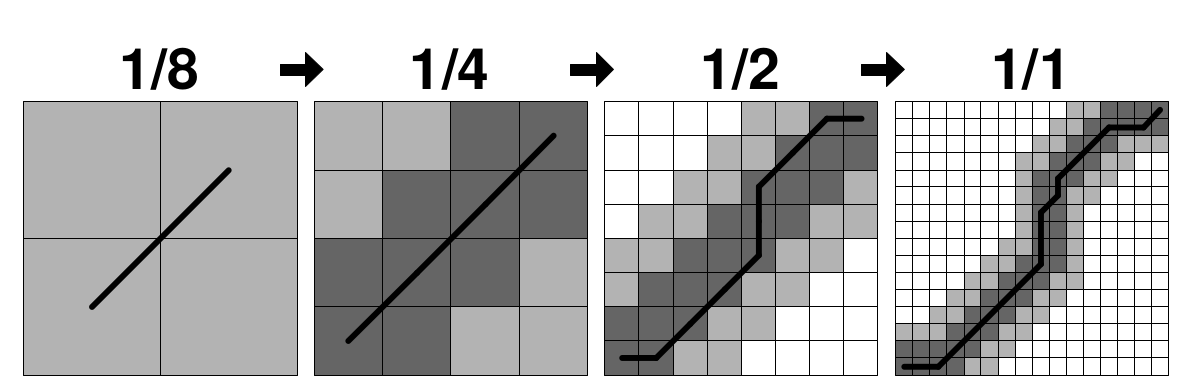
\includegraphics[width=0.9\textwidth]{images/fast_dtw.png}}
  \caption[The four different resolutions evaluated during a complete run of the FastDTW
  algorithm.]{The four different resolutions evaluated during a complete run of the FastDTW
  algorithm.}
  \label{obr:fast_dtw}
\end{figure}

\subsection{Analysis results}

Here we briefly summarize the results of the analysis provided in the original paper
\cite{toward_accurate__dtw}. The algorithm was tested on three different types of sequences and
compared against two other existing approximate DTW algorithms: Sakoe-Chuba \textbf{bands} and
\textbf{data abstraction}.

The FastDTW algorithm is very accurate for all three groups of data that it was tested on. FastDTW
has an error of only $19.2\%$ to $0.0\%$, depending on the value of the radius parameter. For all
algorithms, the error decreases as the radius parameter increases. However, FastDTW converges to
$0\%$ error much faster than the other two algorithms.

\begin{figure}[H]
  \centerline{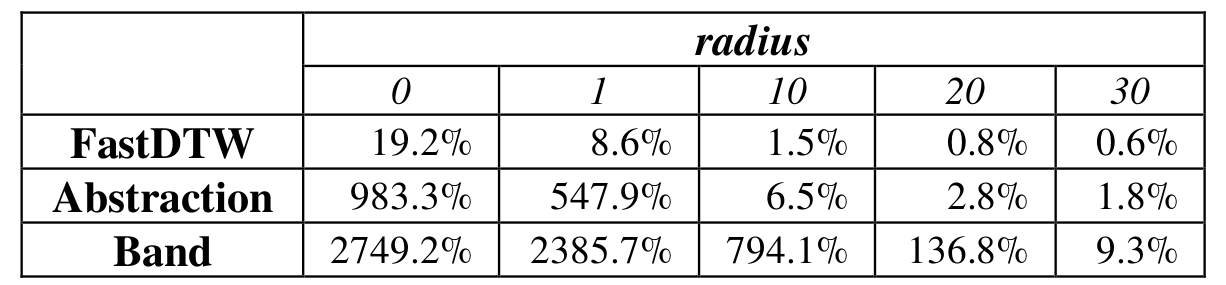
\includegraphics[width=0.9\textwidth]{images/fast_dtw_analysis.png}}
  \caption[Results of accuracy analysis]{Results of accuracy analysis}
  \label{obr:fast_dtw_analysis}
\end{figure}

When we analyze the performance of FastDTW algorithm, the FastDTW algorithm is significantly faster
than the standard DTW algorithm for all but the smallest time series. FastDTW is 50 to 150 times
faster than standard DTW (with $~100$ radius and sequence length of $150000$). You can see a more
detailed results in the table below.

\begin{figure}[H]
  \centerline{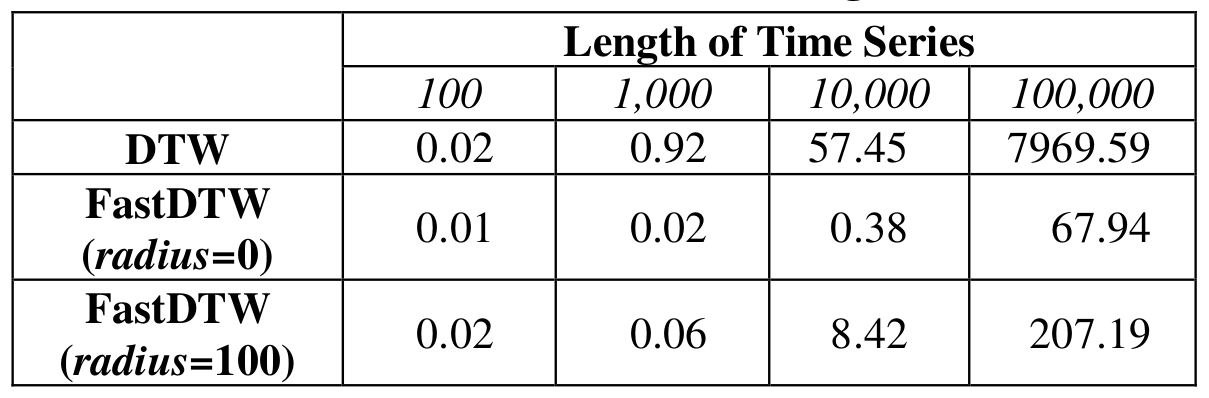
\includegraphics[width=0.9\textwidth]{images/dtw_performance.png}}
  \caption[Results of performance analysis]{Results of performance analysis}
  \label{obr:dtw_performance.png}
\end{figure}

\subsection{FastDTW implementations}

There are many open source implementations of FastDTW algorithm in many different languages like
Java, Python, C++.

\subsection{Disadvantages and further improvements}

The biggest disadvantage of FastDTW algorithm is that it doesn't guarantee an optimal alignment (but
it often does). Further improvements of the algorithm can be by researching how to further increase
the accuracy of the algorithm.
